\subsection{Block-size calculation}

It would be better know that how we calculate the Bitcoin block size based on taproot upgrade now.

\subsubsection{block size}

The block size will be calculated as the following picture:

\begin{figure}[ht] 
    \centering  
    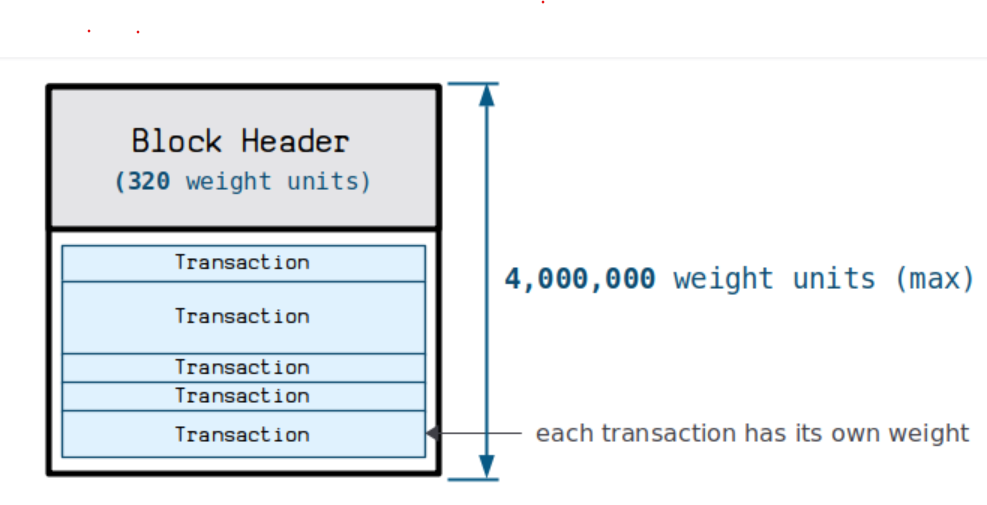
\includegraphics[width=0.85\columnwidth]{images/block-size.png} 
    \caption{Block size}
    \label{fig:block-size}
\end{figure}

\subsubsection{transaction size}

The transaction size will be calculated as the following picture:

\begin{figure}[ht] 
    \centering  
    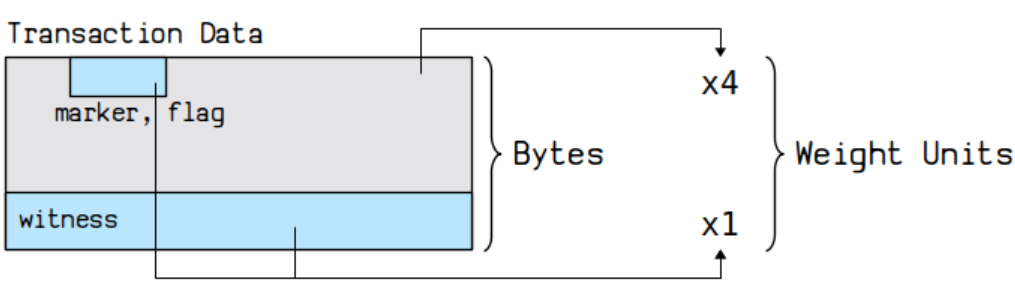
\includegraphics[width=0.85\columnwidth]{images/transaction-size.png} 
    \caption{Transaction size}
    \label{fig:transaction-size}
\end{figure}

You can check more details in \cite{website:transaction-size}

